\section{Results}
\label{sec:results}

This section reports what the framework produced when applied to the two cities. Each scenario is read through the same three indicators — the mean time to the $k$ nearest points of interest (PTh), the inequality of its distribution (index G), and the share of the population served within 15 minutes (F15) — so that the effect of a conditioning layer is measured against a common reference.

Two quantities are kept apart throughout. A conditioning layer either raises the cost of crossing an edge or removes it from the graph, and the two outcomes are not comparable. A cell whose time grew from 8 to 12 minutes remains served, while a cell that lost every path reaches nothing at all. The first is reported as an increase in travel time, the second as loss of access, and averaging them into a single number would hide the difference that matters.

\subsection{Land Surface Temperature as a continuous conditioning layer}
\label{subsec:results-thermal}

In the typical scenario, Curitiba reaches its points of interest quickly. The mean PTh is 8.9 minutes for education, 10.9 for food and 11.6 for health, and F15 stands at 0.921, 0.807 and 0.790 respectively. Averaged across categories, the city reaches its services in 12.6 minutes. Transportation is the exception, with a mean of 19.0 minutes and F15 of 0.565, a value shaped by the density of mapped stops discussed in Section~\ref{subsec:scope-comparison}. The distribution has the shape expected of a compact city, with a well-served core and a periphery where the same services take three to four times longer to reach. The index G runs from 0.270 for education to 0.468 for transportation, with food at 0.350 and health at 0.283.

Applying the thermal layer moves these numbers by little in aggregate. The overall PTh rises from 12.6 to 13.1 minutes, F15 falls from 0.771 to 0.747 on average across categories, and the index G changes by less than 0.005 in every one of them. The median increase in travel time is half a minute, with a 90th percentile of one minute. Every cell keeps its access, because the thermal factor multiplies the cost of an edge and leaves the graph connected.

The aggregate is modest because the calibrated factor is modest. The composite surface temperature of Curitiba spans 12.9 to 38.2~°C, and the calibrated slope converts that range into factors between 1.00 and 1.11; at the hottest pixel in the city, a route becomes 11\% more expensive. Figure~\ref{fig:results-curitiba} shows that this small average conceals a spatial pattern. The third panel is nearly white in the centre and dark in the western and southern periphery, where the surface temperature is highest and the network is sparsest. The layer shifts the city where heat and distance coincide, and leaves it unchanged elsewhere.

\begin{figure}[htbp]
  \centering
  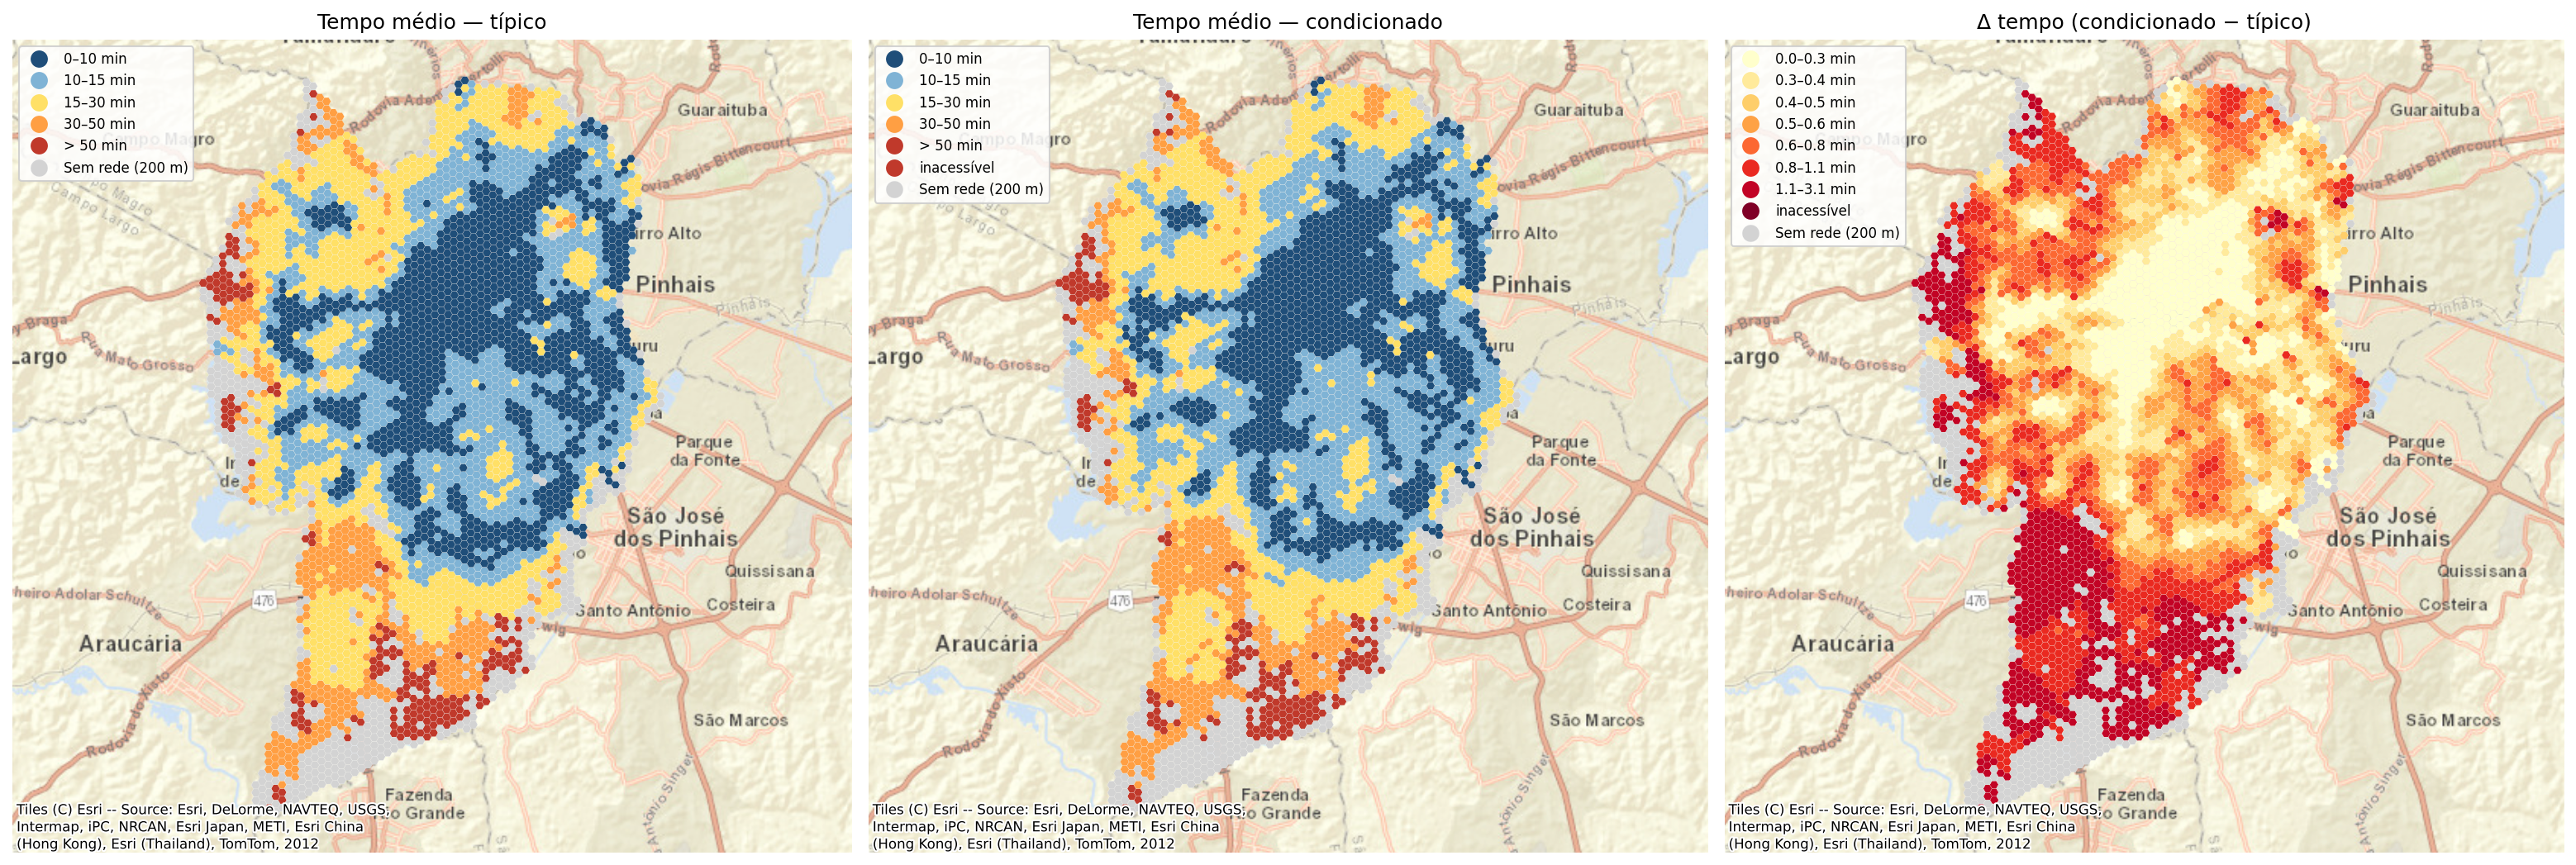
\includegraphics[width=1\textwidth]{figs/curitiba_lst.png}
  \caption{Curitiba under the thermal scenario. Left: mean access time in the typical scenario. Centre: the same cells after the thermal factor is applied. Right: the per-cell increase in access time, in minutes; grey cells lie beyond the snapping threshold and carry no pedestrian network. The increase concentrates in the western and southern periphery while the centre remains nearly unchanged.}
  \label{fig:results-curitiba}
\end{figure}

The \texttt{thermal\_demo} scenario, which uses a slope seven times the calibrated one, shows what the same mechanism produces when the gradient is steeper. The overall PTh rises to 16.3 minutes and F15 falls from 0.771 to 0.600, the median increase reaches 3.6 minutes and the worst cell gains 21.5 minutes. The spatial pattern keeps its shape and intensifies. The layer is read, sampled and applied identically in both runs, and only the coefficient differs, which isolates the behaviour of the mechanism from the magnitude of the calibration.

Adding vegetation reverses part of the effect. Under \texttt{thermal+green} the overall PTh returns to 13.0 minutes, the F15 loss falls from 2.4 to 1.8 points measured against the typical scenario, and the median increase drops from 0.51 to 0.36 minutes. The vegetation factor multiplies the thermal one at the same sampled point, so the reduction applies to the temperature of the sidewalk that carries the shade. That is what the composite arrangement exists to guarantee.

Figure~\ref{fig:results-curitiba-vegetation} shows the same spatial pattern with lower intensity. The darkest classes thin out where the tree cover is densest, and the centre loses part of its residual delay. Vegetation removes a share of the increase wherever heat was measured, so the geography of the effect is unchanged and only its intensity falls.

\begin{figure}[htbp]
  \centering
  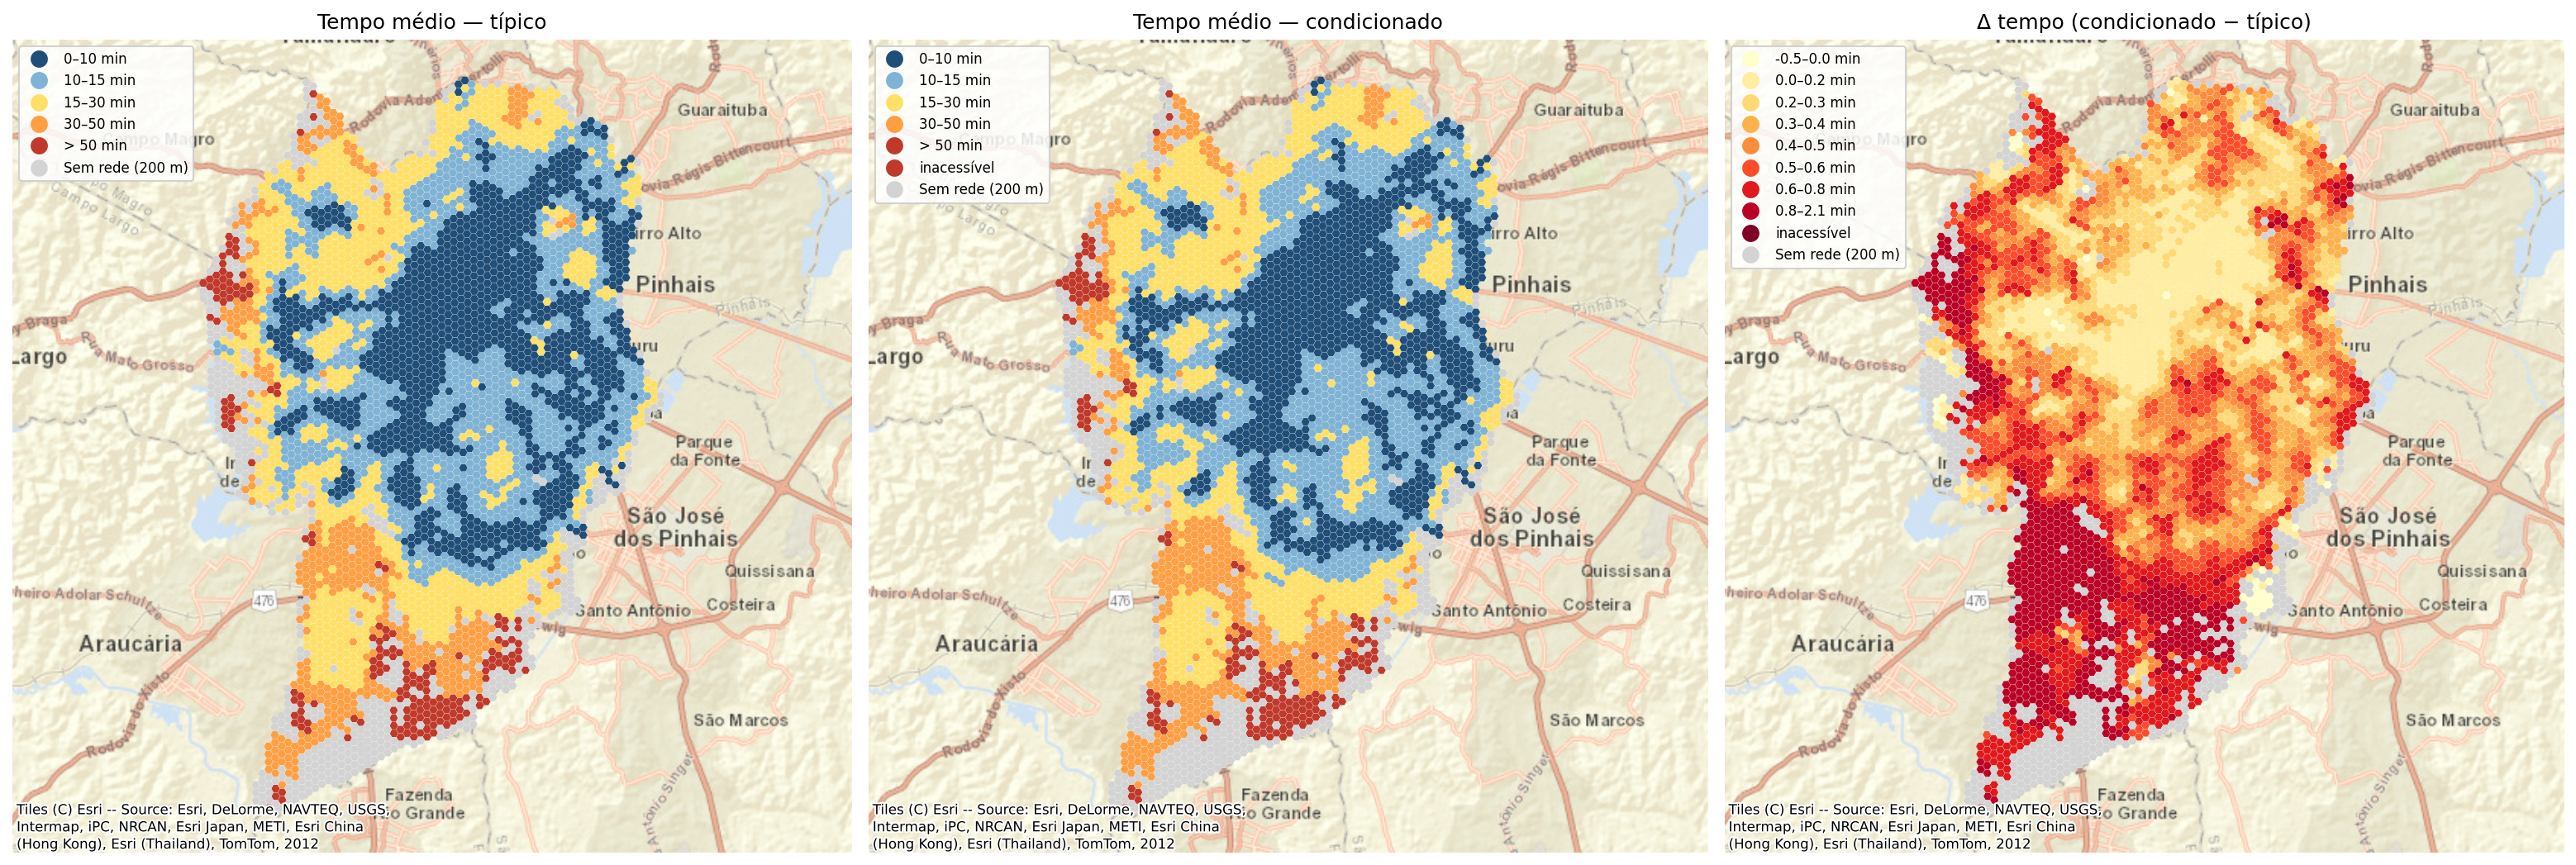
\includegraphics[width=1\textwidth]{figs/curitiba_green.png}
  \caption{Curitiba under the \texttt{thermal+green} scenario. Left: mean access time in the typical scenario. Centre: the same cells after the composite factor is applied. Right: the per-cell increase in access time, in minutes; the classes are narrower than in Figure~\ref{fig:results-curitiba} because the shade reduces the thermal penalty. Grey cells lie beyond the snapping threshold and carry no pedestrian network.}
  \label{fig:results-curitiba-vegetation}
\end{figure}

\subsection{Flood and landslide as discrete conditioning layers}
\label{subsec:results-flood}

The typical scenario in Porto Alegre reaches education in 9.4 minutes, food in 12.4 and health in 14.3, with F15 at 0.857, 0.728 and 0.673. Averaged across categories, the city reaches its services in 15.1 minutes, against 12.6 in Curitiba. The index G is 0.352 for education, 0.380 for food, 0.431 for health and 0.305 for transportation, and the dispersion is wider than in Curitiba. Among the cells that do reach a health facility, the slowest tenth takes more than 87.8 minutes, against 34.5. Transportation again departs from the pattern, with a mean of 24.0 minutes and F15 of 0.221, consistent with the sparse mapping of stops noted in Section~\ref{subsec:scope-comparison}.

The \texttt{flood} scenario raises the overall PTh from 15.1 to 20.7 minutes and lowers F15 from 0.620 to 0.510, with a median cell increase of 3.3 minutes and a 90th percentile of 46 minutes. No cell loses access, because the factor is finite and only multiplies the cost of the edge, leaving the graph connected. The magnitude far exceeds the thermal case because the factor is far larger. The three risk classes carry factors of 1.71, 1.86 and 2.14, applied to a flooded area of 250.8~km$^2$, which is 47.6\% of the municipality. Figure~\ref{fig:results-porto-alegre-flood} presents the resulting access times and the corresponding changes across cells.

\begin{figure}[htbp]
  \centering
  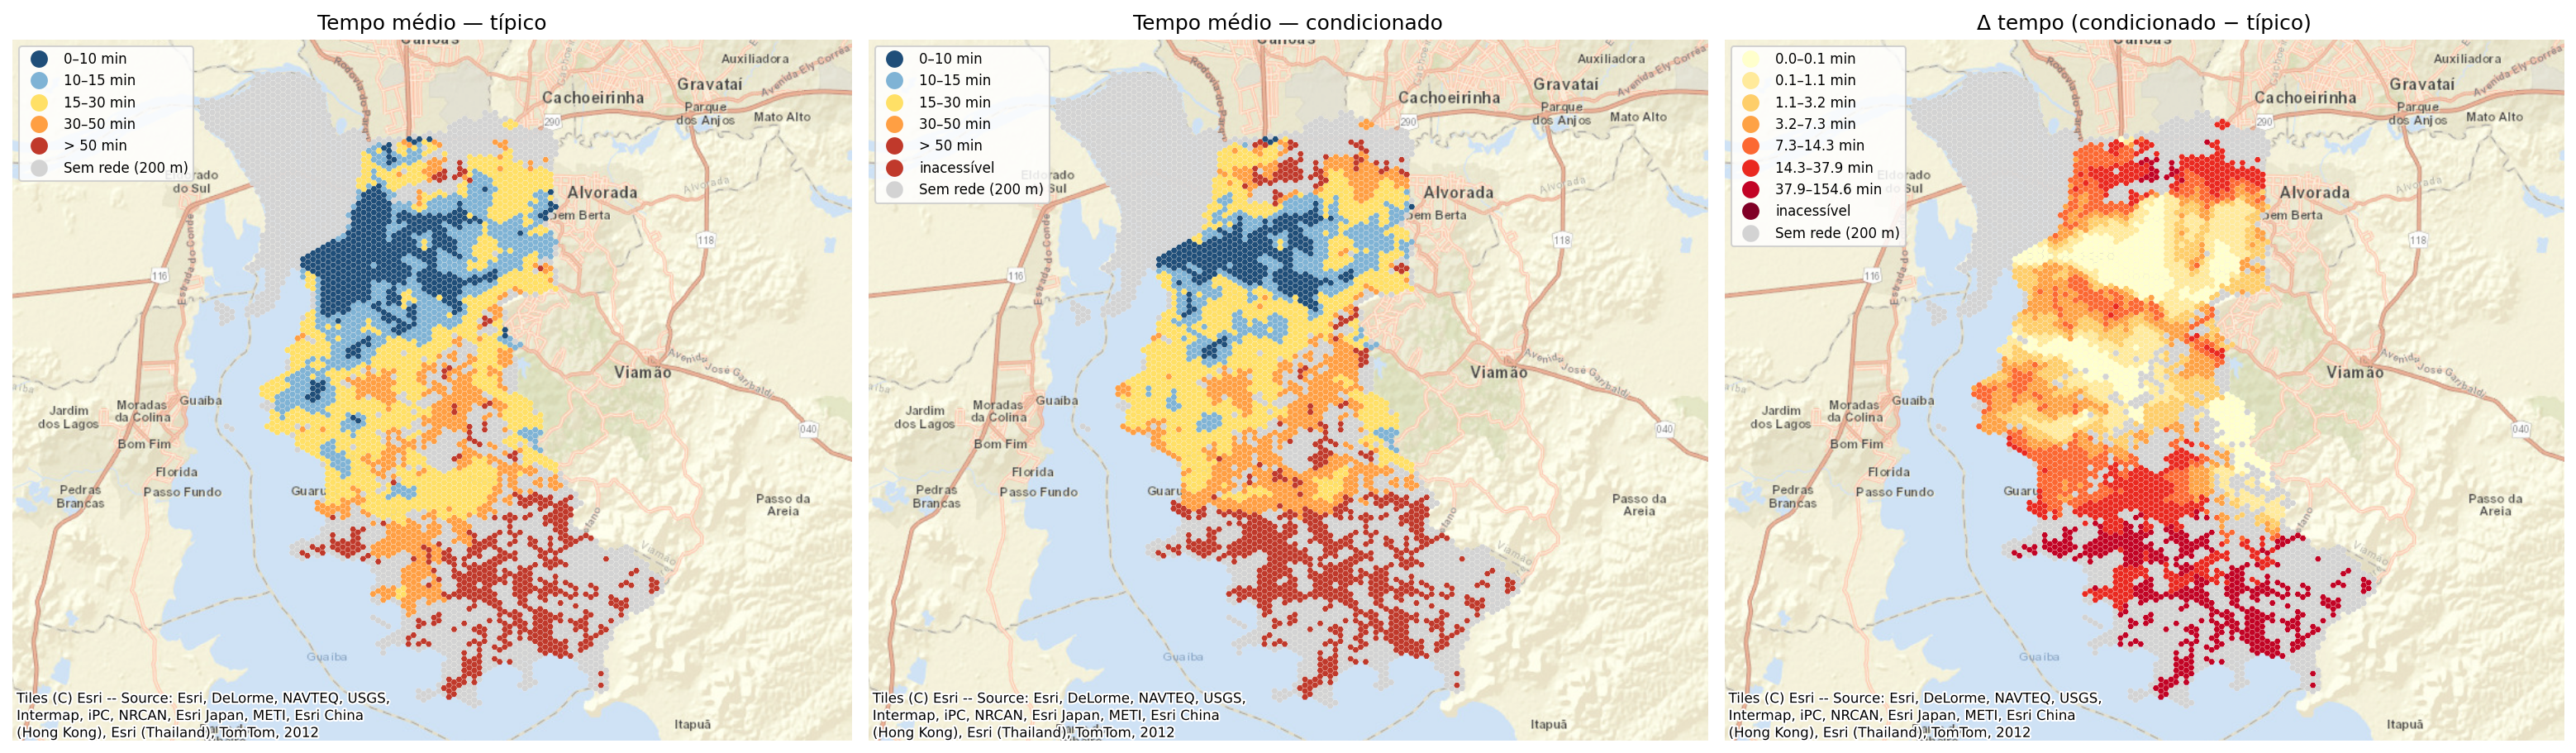
\includegraphics[width=1\textwidth]{figs/porto_alegre_inundacao.png}
  \caption{Porto Alegre under the \texttt{flood} scenario. Left: mean access time in the typical scenario. Centre: the same cells after the flood factor is applied. Right: the per-cell increase in access time, in minutes. The delay covers the floodplain and tapers towards the edges of the affected polygons; no cell loses network.}
  \label{fig:results-porto-alegre-flood}
\end{figure}

The \texttt{landslide} scenario removes 9{,}465 of the 36{,}780 cell--POI pairs from reach, or 25.7\% of the matrix, and leaves every other pair untouched. The median increase among the pairs that survive is zero, because a cell outside the mapped polygons keeps its original cost. An infinite factor therefore produces a different outcome from a finite one, and the framework reports it separately. In the figure, a cell inside the affected polygons either falls in a delay class or is drawn in red, the top of the scale, which marks loss of access; grey marks cells beyond the snapping threshold, which never enter the matrix. Figure~\ref{fig:results-porto-alegre} shows the two outcomes together.

\begin{figure}[htbp]
  \centering
  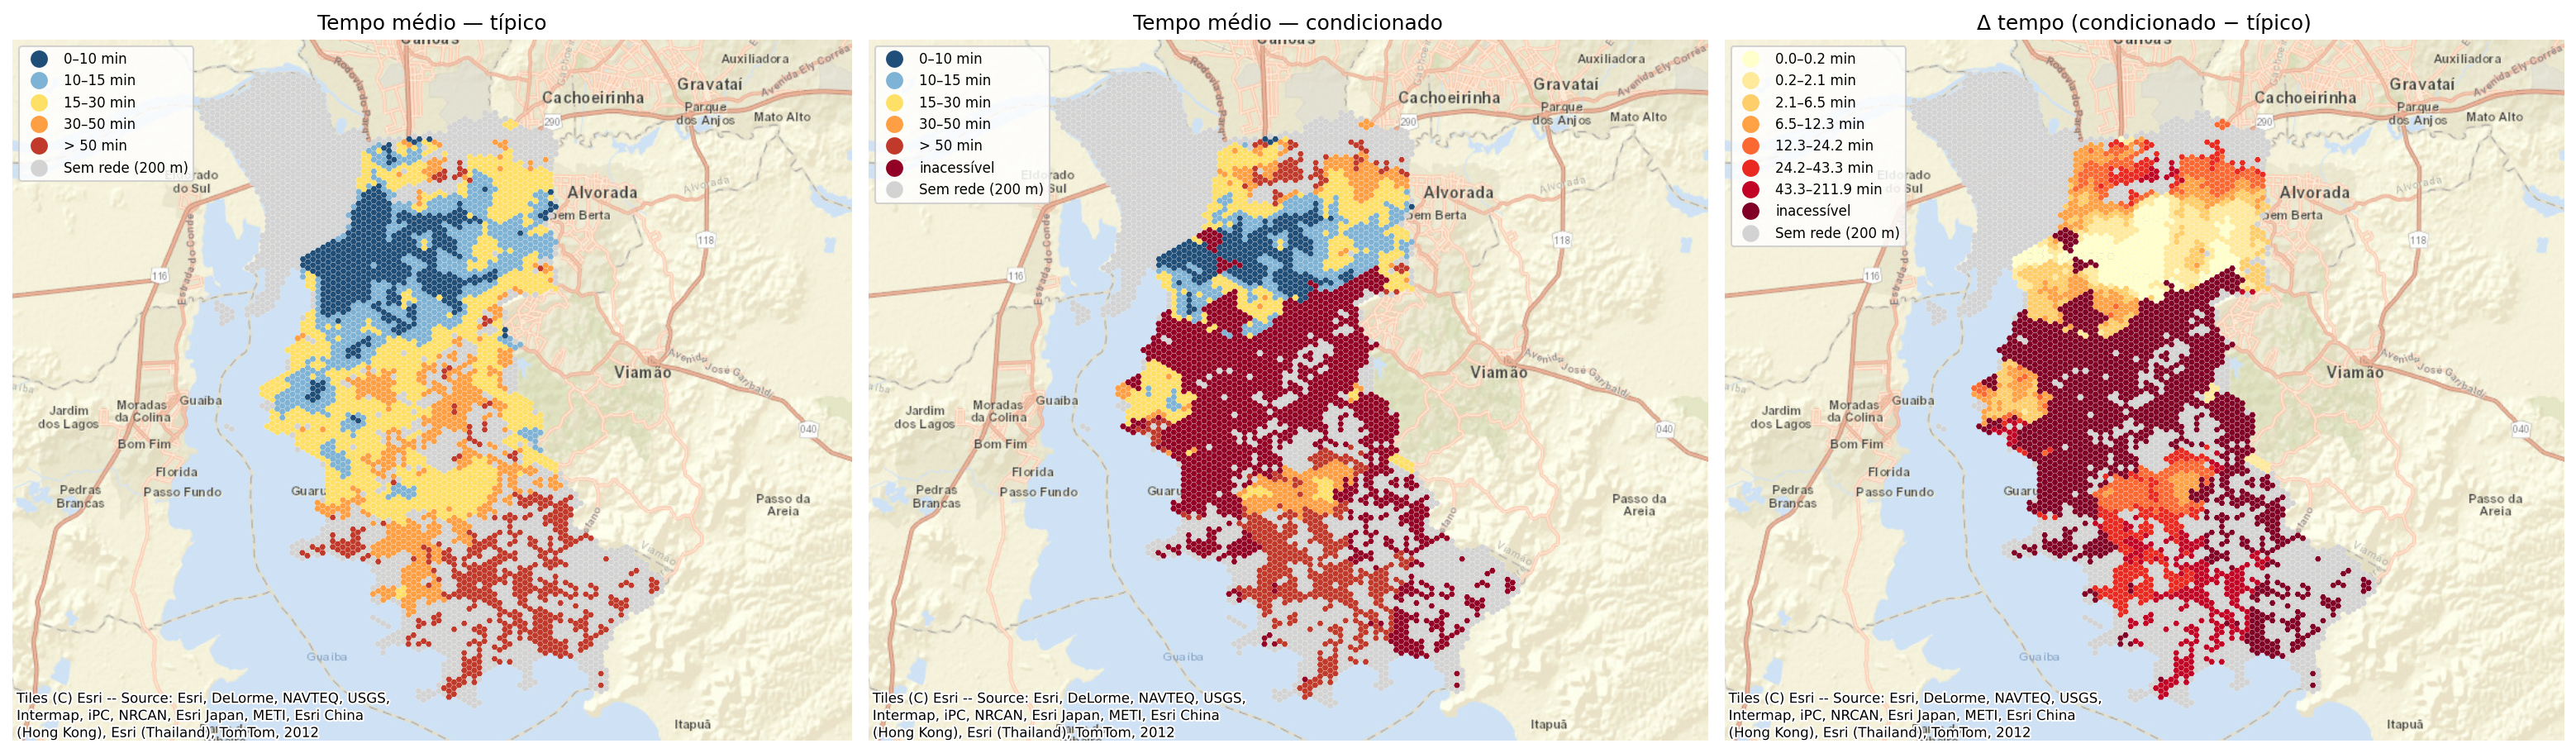
\includegraphics[width=1\textwidth]{figs/porto_alegre_combinado.png}
  \caption{Porto Alegre under the \texttt{flood+landslide} scenario. Left: mean access time in the typical scenario. Centre: the same cells after both layers are applied, with loss of access drawn in red at the top of the scale. Right: the per-cell increase in access time, in minutes. Grey marks cells beyond the snapping threshold, which carry no pedestrian network. The two hazards leave different marks, as flooding shades a broad area while landsliding removes whole cells from the reachable set.}
  \label{fig:results-porto-alegre}
\end{figure}

\subsection{How layers combine in each case}
\label{subsec:results-composition}

Combining the two layers in Porto Alegre, as in \texttt{flood+landslide}, does not add their effects. The number of pairs that lose access is the same as under \texttt{landslide} alone, 9{,}465, which confirms that the infinite factor dominates any finite one on a shared edge. What changes is the set of cells that remain connected and the cost of their paths. Under \texttt{landslide} the 2{,}446 cells that keep every destination pay nothing, because their shortest routes never cross an interdicted polygon. Restricting both scenarios to those same 2{,}446 cells, the median increase goes from 5.2 to 6.4 minutes and the 90th percentile from 49 to 81. The delay each cell already carried is compounded by the detour around the blocked polygons, and the 619 cells that lose access to every point of interest are counted separately, entering neither statistic.

The composite arrangement in Curitiba shows the same property from the other side. Chaining two simple rules would apply the vegetation discount to any tree-lined segment, including the ones where the thermal factor is already at its floor of 1, and to segments whose temperature was sampled at a different position along the edge. Reading both layers at identical points keeps the discount tied to the shade actually present where the heat was measured. The result is a reduction of the F15 loss from 2.4 to 1.8 points, measured against the typical scenario.

\subsection{Socioeconomic distribution of the change}
\label{subsec:results-socioeconomic}

The aggregate change is small in Curitiba and large in Porto Alegre, and in both cities it is unevenly distributed. Spearman correlations between each axis of the deprivation index and the per-cell increase are positive and significant in every scenario and city (Table~\ref{tab:results-correlation}), which means the cells that lose the most time are also the cells with worse sanitation, lower income and higher illiteracy.

\begin{table}[htbp]
\centering
\caption{Spearman correlation between each axis of the socioeconomic deprivation index and the per-cell increase in access time. All coefficients are significant at $p < 0.001$.}
\label{tab:results-correlation}
\footnotesize
\begin{tabular}{llrrrr}
\hline
City & Scenario & Sanitation & Income & Illiteracy & Composite \\
\hline
Curitiba & \texttt{thermal} & 0.350 & 0.357 & 0.306 & 0.449 \\
Curitiba & \texttt{thermal\_demo} & 0.351 & 0.356 & 0.305 & 0.449 \\
Curitiba & \texttt{thermal+green} & 0.098 & 0.442 & 0.300 & 0.332 \\
Curitiba & \texttt{thermal+green\_demo} & 0.330 & 0.374 & 0.312 & 0.446 \\
Porto Alegre & \texttt{flood} & 0.307 & 0.178 & 0.208 & 0.278 \\
Porto Alegre & \texttt{landslide} & 0.198 & 0.105 & 0.165 & 0.181 \\
Porto Alegre & \texttt{flood+landslide} & 0.530 & 0.336 & 0.398 & 0.504 \\
\hline
\end{tabular}
\end{table}

The composite index and its axes rank the cells differently in each city. In Curitiba the composite carries a higher correlation than any single axis in the two plain thermal scenarios, at 0.449 against 0.357 for income, because the three axes capture different sides of the same condition and their sum separates the affected cells better than each one separately. Adding vegetation breaks that relation. Under \texttt{thermal+green} income alone reaches 0.442 and sanitation falls to 0.098, so the composite drops to 0.332, below the highest axis. The vegetation layer removes the delay from the shaded segments, and the sanitation axis, which described where the heat was mapped, loses its grip on the change in the same movement.

Porto Alegre shows the opposite ordering. Sanitation carries the highest correlation of the three axes in every scenario, at 0.530 under \texttt{flood+landslide}, 0.307 under \texttt{flood} and 0.198 under \texttt{landslide}. The composite stays below it in all three, because income and illiteracy are weakly associated with the change and dilute the signal when given equal weight. The gap widens under the two layers together, where sanitation rises to 0.530 while income falls to 0.336 and illiteracy to 0.398.

\subsection{Simultaneous regression}
\label{subsec:results-regression}

Correlations treat each axis on its own; a regression with the three axes as simultaneous predictors separates the contribution of each once the others are held. The dependent variable is the per-cell increase in access time, not the level of access, so the coefficients describe who absorbs the delay and not who was already poorly served. Table~\ref{tab:results-regression} reports the standardized coefficients, which express each axis in standard deviations of both the axis and the outcome, so that axes measured on different scales become comparable.

\begin{table}[htbp]
\centering
\caption{Standardized coefficients of the regression of per-cell median access time increase on the three axes of the deprivation index, and variance inflation factors of the same model. All coefficients significant at $p < 0.01$ except those marked.}
\label{tab:results-regression}
\footnotesize
\begin{tabular}{llrrrrr}
\hline
City & Scenario & Sanitation & Income & Illiteracy & Adj.\ $R^2$ & VIF \\
\hline
Curitiba & \texttt{thermal} & $0.382$ & $0.331$ & $-0.163$ & 0.205 & 1.18--1.87 \\
Curitiba & \texttt{thermal\_demo} & $0.383$ & $0.330$ & $-0.162$ & 0.206 & 1.18--1.87 \\
Curitiba & \texttt{thermal+green} & $0.111$ & $0.436$ & $-0.147$ & 0.146 & 1.18--1.87 \\
Curitiba & \texttt{thermal+green\_demo} & $0.360$ & $0.346$ & $-0.161$ & 0.200 & 1.18--1.87 \\
Porto Alegre & \texttt{flood} & $0.375$ & $0.006^{*}$ & $0.051$ & 0.170 & 1.72--2.25 \\
Porto Alegre & \texttt{landslide} & $0.163$ & $-0.036^{*}$ & $0.055^{*}$ & 0.032 & 1.78--2.40 \\
Porto Alegre & \texttt{flood+landslide} & $0.420$ & $-0.047^{*}$ & $0.104$ & 0.215 & 1.78--2.40 \\
\hline
\multicolumn{7}{l}{\footnotesize $^{*}$not significant at $p < 0.05$.} \\
\end{tabular}
\end{table}

In Curitiba the sanitation and income coefficients are positive and the illiteracy coefficient is negative, $-0.163$ in the thermal scenario, with an adjusted $R^2$ of 0.205. The variance inflation factors stay between 1.18 and 1.87, far below the threshold of 5, so collinearity does not explain the reversal. Once sanitation and income are held fixed, illiteracy marks the denser and better-connected tracts, where a high-illiteracy tract in the centre still has alternative routes when its edges are penalized and loses less time than a tract with the same illiteracy in the periphery.

Adding vegetation changes which axis carries the relation. Under \texttt{thermal+green} the sanitation coefficient falls from $0.382$ to $0.111$, the income coefficient rises from $0.331$ to $0.436$, and the explained variance drops from 0.205 to 0.146. The attenuation is concentrated where the thermal penalty is strongest, and the vegetation layer removes part of the time increase from exactly those segments, so the axis that described where the heat was mapped loses part of its grip on the outcome. What remains explaining the change is income, now the dominant axis. The cells that keep losing time are the poor ones that the tree cover does not reach.

Porto Alegre behaves differently. Under \texttt{flood}, sanitation takes $0.375$ and the other two axes fall to 0.006 and 0.051, the first of them not significant. One axis absorbs almost all the explained variance, adjusted $R^2$ of 0.170. Under \texttt{landslide}, the coefficients collapse together, adjusted $R^2$ of 0.032, income and illiteracy not significant, and only sanitation retains $0.163$. An interdiction by polygon removes cells from the matrix according to where the slope is, a criterion the deprivation index does not see. Under \texttt{flood+landslide}, sanitation reaches $0.420$, the highest coefficient in the table, with adjusted $R^2$ of 0.215. A cell without adequate sanitation in a flood-prone area is both more likely to be inundated and less likely to have an alternative route, and the two conditions compound.

\subsection{Spatial clusters}
\label{subsec:results-lisa}

The regression treats cells as independent, which they are not. The bivariate Moran statistic provides the global test, and it rejects that independence in every scenario. In Curitiba $I = 0.373$ under \texttt{thermal}, and in Porto Alegre $0.362$ under \texttt{flood} and $0.410$ under \texttt{flood+landslide}, all at $p = 0.001$. Adding vegetation lowers the global statistic in Curitiba to $0.258$ under \texttt{thermal+green}$, and adding landsliding lowers it in Porto Alegre to $0.165$ under \texttt{landslide}$, which is what the drop in explained variance already indicated.

The local indicators locate where that association sits. They separate the cells whose value of the SDI and whose time increase are both high (High-High) or both low (Low-Low) from the two discordant classes, high deprivation with low increase (High-Low) and low deprivation with high increase (Low-High). Cells not significant at $p \le 0.05$ receive no class. Table~\ref{tab:results-lisa} gives the share of the grid in each class.

\begin{table}[htbp]
\centering
\caption{Share of cells in each local bivariate cluster between the SDI and the per-cell increase in access time, as percentage of the grid. Global Moran $I$ and the share of significant cells are given for each scenario.}
\label{tab:results-lisa}
\fontsize{9}{9.6}\selectfont
\setlength{\tabcolsep}{4pt}
\begin{tabular}{llrrrrrr}
\hline
City & Scenario & Moran $I$ & Sig.\ (\%) & High-High & Low-Low & High-Low & Low-High \\
\hline
Curitiba & \texttt{thermal} & 0.373 & 37.3 & 7.6 & 20.5 & 5.8 & 3.3 \\
Curitiba & \texttt{thermal+green} & 0.258 & 35.1 & 8.4 & 16.5 & 6.4 & 3.8 \\
Curitiba & \texttt{thermal+demo} & 0.373 & 36.5 & 7.3 & 20.1 & 5.8 & 3.3 \\
Curitiba & \texttt{thermal+green+demo} & 0.369 & 37.0 & 8.2 & 19.9 & 5.6 & 3.3 \\
Porto Alegre & \texttt{flood} & 0.362 & 50.6 & 11.4 & 19.6 & 18.9 & 0.7 \\
Porto Alegre & \texttt{landslide} & 0.165 & 51.7 & 2.9 & 11.6 & 36.6 & 0.6 \\
Porto Alegre & \texttt{flood+landslide} & 0.410 & 43.7 & 8.8 & 22.3 & 12.3 & 0.3 \\
\hline
\end{tabular}
\end{table}

\begin{figure}[htbp]
\centering
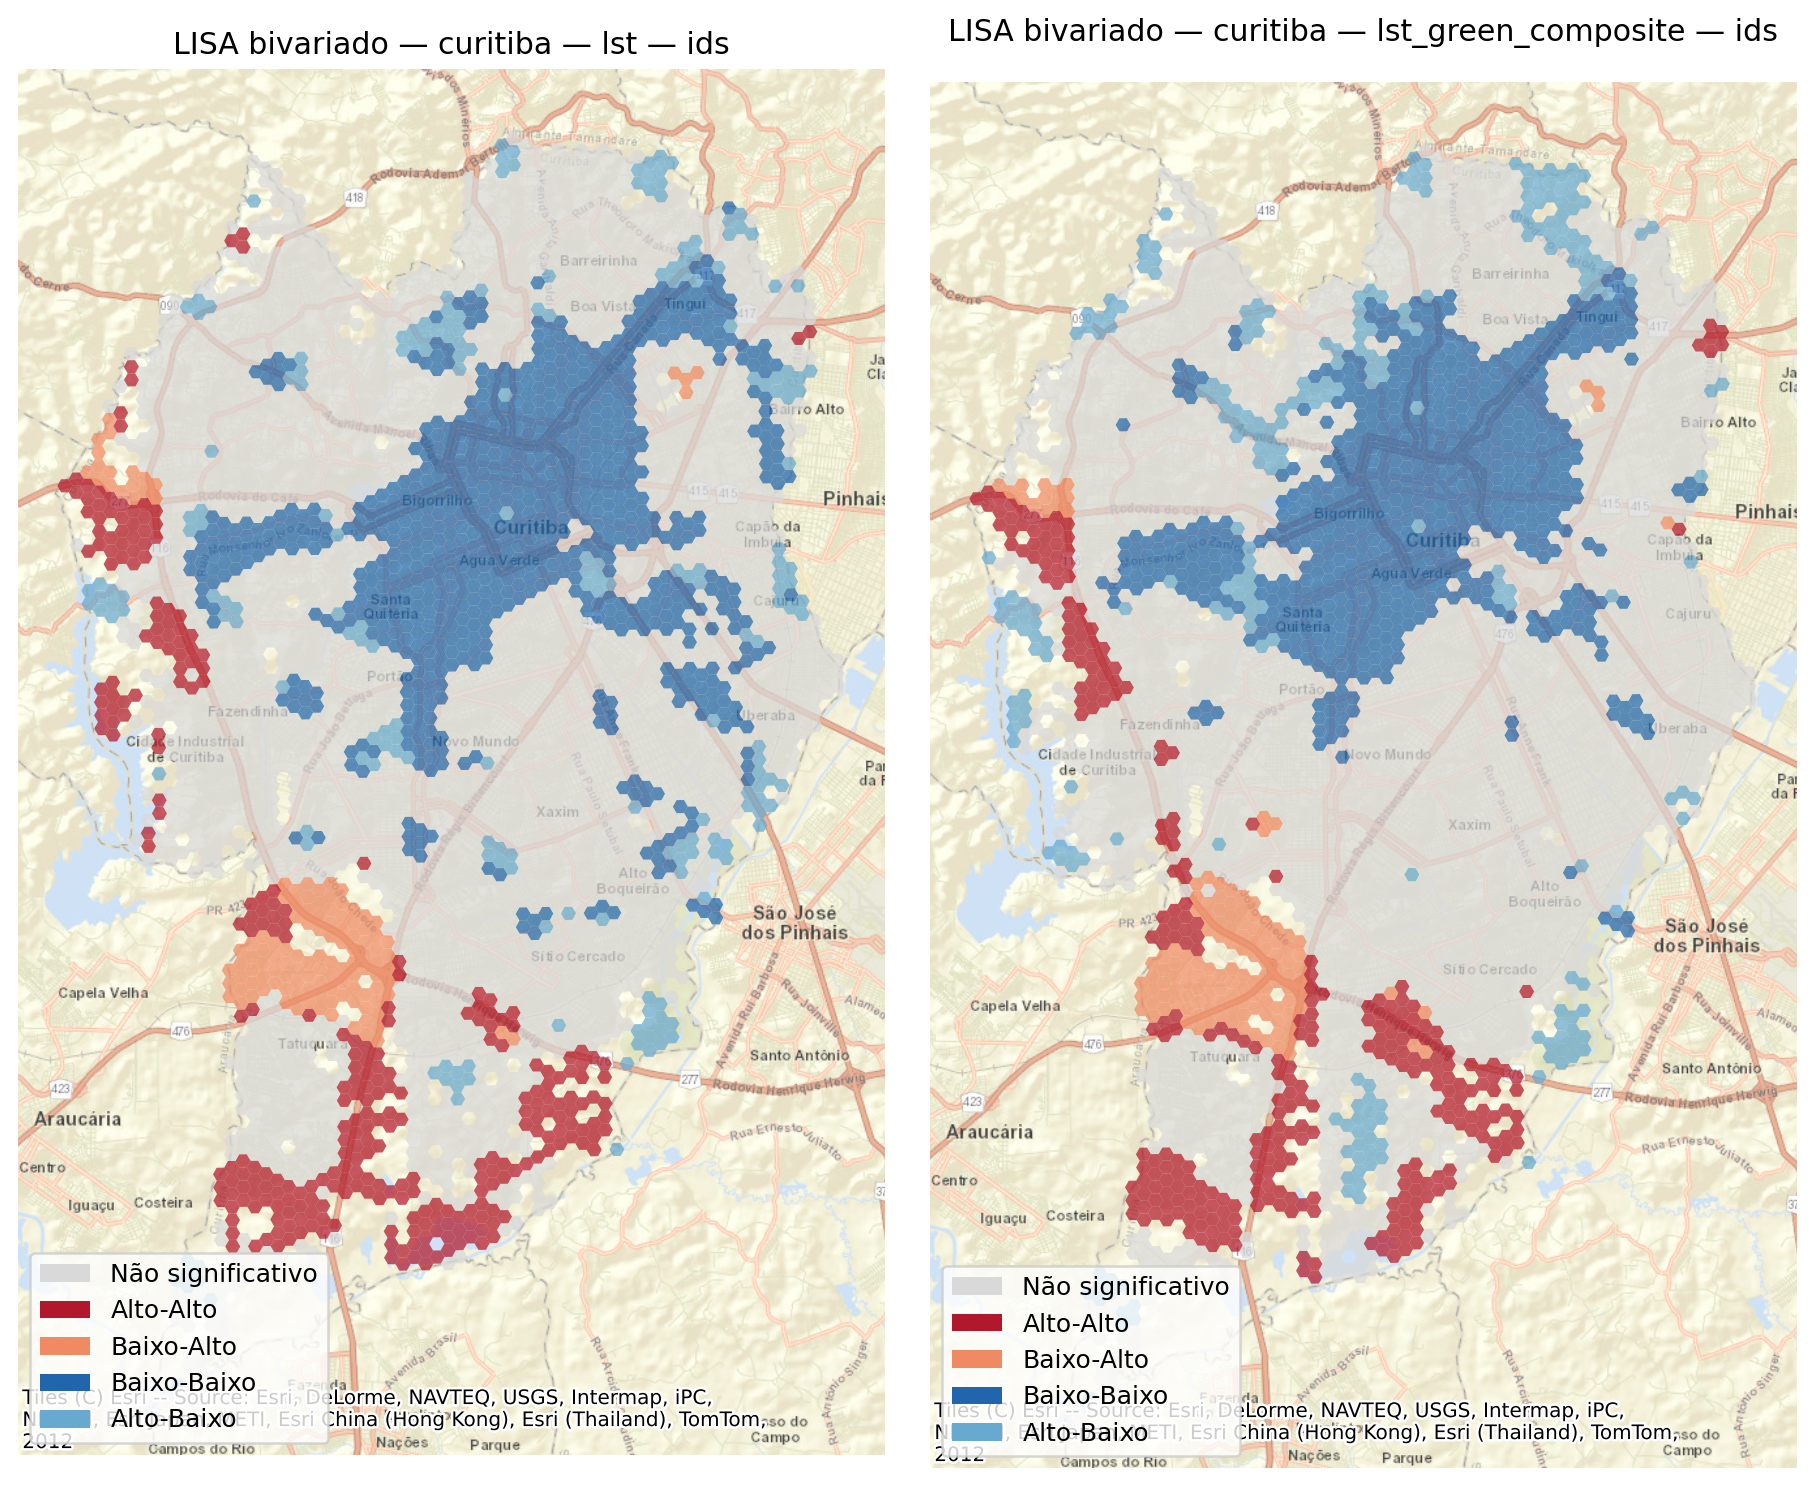
\includegraphics[height=0.30\textheight]{figs/lisa_curitiba.png}
\caption{Local bivariate clusters between the SDI and the per-cell increase in access time, Curitiba, under \texttt{thermal} (left) and \texttt{thermal+green} (right). Grey cells are not significant at $p \le 0.05$.}
\label{fig:results-lisa-curitiba}
\end{figure}

In Curitiba (Figure~\ref{fig:results-lisa-curitiba}), the Low-Low class accounts for 16.5\% of the grid under \texttt{thermal+green} against 8.4\% in High-High. That asymmetry reproduces the aggregate result. The large continuous core of the city has both low deprivation and no time increase, while the High-High clusters form separate patches at the western edge and along the southern corridor, where the two conditions coincide. The clusters that remain under \texttt{thermal+green} overlap the tracts the tree cover does not reach, which is the income axis doing the work the regression attributed to it. The vegetation also thins the Low-Low core from 20.5\% under \texttt{thermal} to 16.5\%, as the shade removes part of the delay from the centre and some central cells fall back under the significance threshold.

\begin{figure}[htbp]
\centering
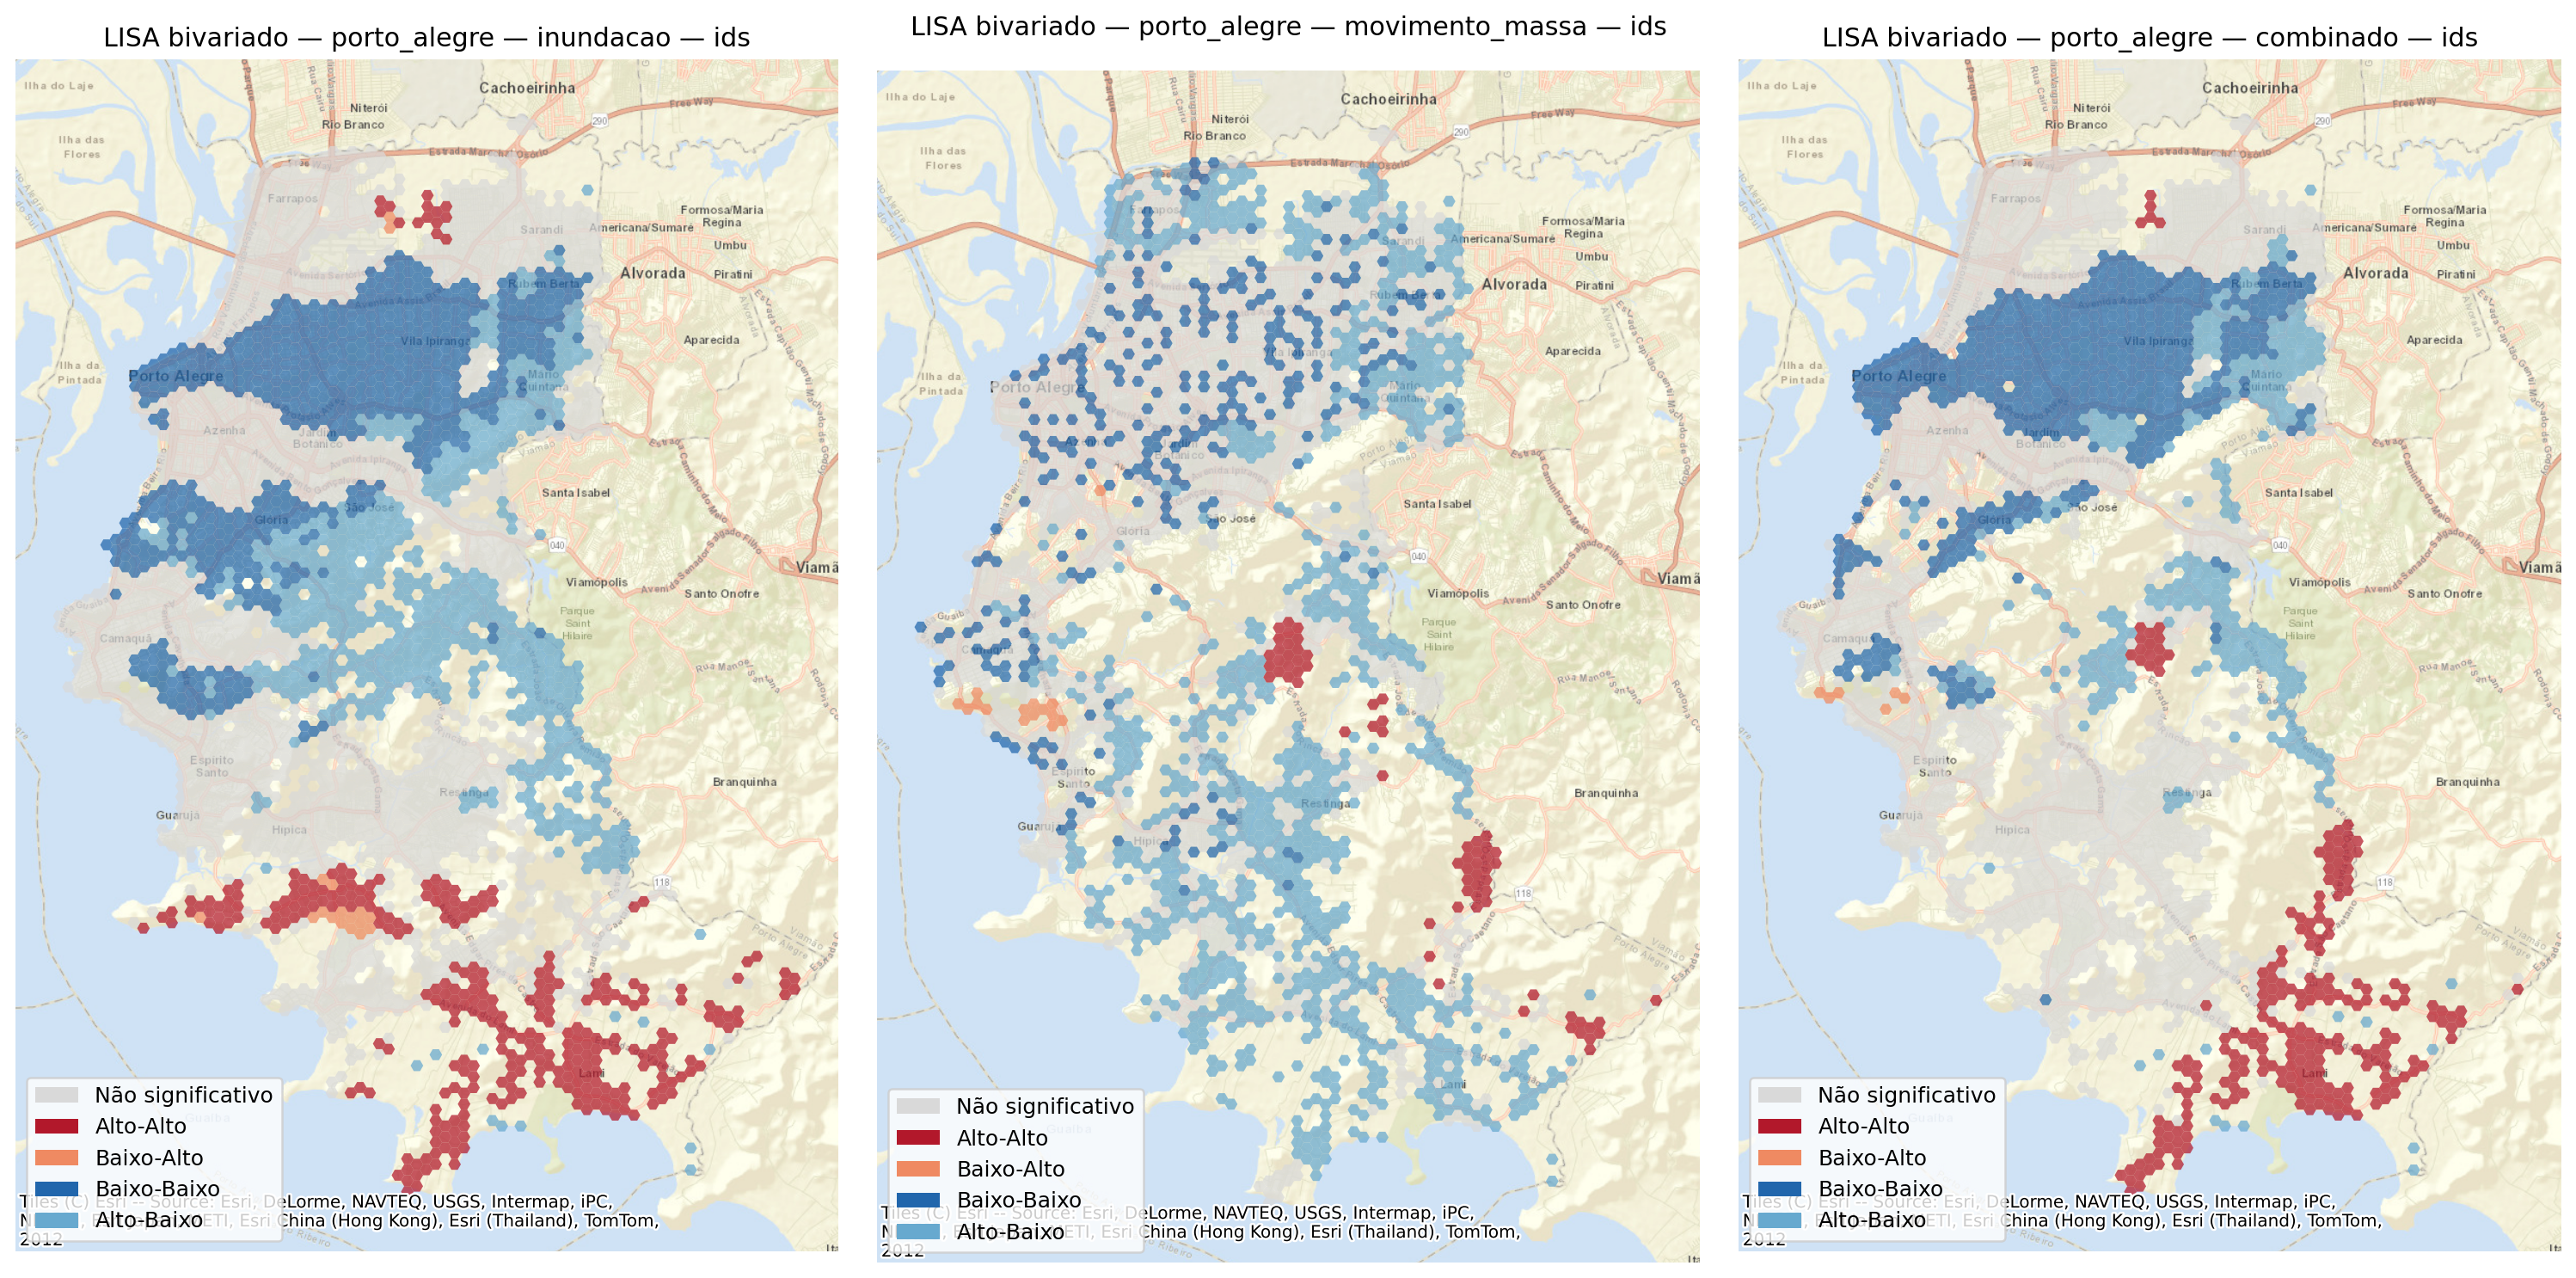
\includegraphics[height=0.26\textheight]{figs/lisa_porto_alegre.png}
\caption{Local bivariate clusters between the SDI and the per-cell increase in access time, Porto Alegre, under \texttt{flood} (left), \texttt{landslide} (centre) and \texttt{flood+landslide} (right). Grey cells are not significant at $p \le 0.05$.}
\label{fig:results-lisa-porto-alegre}
\end{figure}

Porto Alegre produces a signature the global statistic alone would hide (Figure~\ref{fig:results-lisa-porto-alegre}). Under \texttt{flood}, High-Low reaches 18.9\% of the cells, as large as the 19.6\% of Low-Low. Cells inside the floodplain lose time because the inundation reaches them by the polygon. Under \texttt{landslide} the same class grows to 36.6\%, and High-High falls to 2.9\%. The slope polygons intersect the city where deprivation is low, so \texttt{landslide} in this municipality concentrates loss of access in the better-served areas. Under \texttt{flood+landslide} the classes rebalance, High-High at 8.8\% and Low-Low at 22.3\%, and the High-High clusters become contiguous along the southern periphery, which is the pattern of a compound exposure acting on a network whose service provision already follows the same gradient.

Taken together, the results show the mechanism responding to the three properties the scenarios were built to exercise. It distinguishes continuous from discrete evidence, it distinguishes a delay from an interruption, and it composes layers without collapsing them into an average. Whether the magnitudes correspond to what would be observed in an actual event is a question the scenarios do not answer, and the next section takes it up.

